\chapter{软间隔支持向量机}

\section{处理噪声数据}

硬间隔支持向量机最大的问题是它要求数据是线性可分的。现实生活中的数据常常是线性不可分的。即使数据是线性可分的,在将其输入模型之前也会发生很多事情。也许有人在示例中输入了错误的值,或者可能传感器的探测返回了一个异常的值。在存在异常值(离该类别的大部分数据点很远)的情况下,有两种情况:异常值可以比该类的大多数样本更接近其他类别的样本,从而导致间隔的减少,或者它打破其他类别的线性可分性。 让我们硬间隔SVM是如何处理这两种情况的。

\subsection{异常值减小间隔}

当数据线性可分时,硬间隔分类器在存在异常值时不会像我们希望的那样。

现在让我们考虑添加异常数据点(5,7)的数据集,如图\ref{figure33}所示。

\begin{figure}[ht]
	\centering
	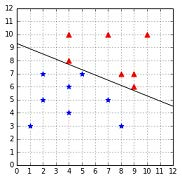
\includegraphics{figure33}
	\caption{添加异常点(5,7)后,数据依然是线性可分的}
	\label{figure33}
\end{figure}

在本例中,我们可以看到间隔非常窄,似乎异常值是这一变化的主要原因。直观地,我们可以看到这个超平面可能不是分离数据的最佳超平面,而且它的泛化能力可能很差。

\subsection{异常值让数据线性不可分}

更糟糕的是,当异常值打破线性可分性时,如图\ref{figure34}中的点(7,8),分类器无法找到超平面。我们被一个单一的数据点卡住了

\begin{figure}[ht]
	\centering
	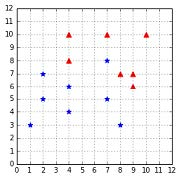
\includegraphics{figure34}
	\caption{异常点(7,8)让数据线性不可分}
	\label{figure34}
\end{figure}


\section{软间隔代解决方案}

\subsection{松弛变量}

1995年,Vapnik和Cortes引入了原始支持向量机的改进版本,允许分类器犯一些错误。现在的目标不是零分类错误,而是犯尽可能少的错误。

为此,他们通过添加一个变量$\zeta$(zeta)来修改优化问题的约束条件。约束:
\begin{gather*}
y_i (\mathbf{w}\cdot \mathbf{x}_i + b) \geq 1
\end{gather*}
变成了:
\begin{gather*}
y_i (\mathbf{w}\cdot \mathbf{x}_i + b) \geq 1-\zeta_i
\end{gather*}

因此,在最小化目标函数时,即使样本不满足原始约束(即离超平面太近,或不在超平面的正确一侧),也有可能满足该约束。代码29说明了这一点。

\emph{代码29}

\begin{lstlisting}[language=python]
import numpy as np 

w = np.array([0.4, 1]) 
b = -10 

x = np.array([6, 8]) 
y = -1 

def constraint(w, b, x, y): 
    return y * (np.dot(w, x) + b)

def hard_constraint_is_satisfied(w, b, x, y): 
    return constraint(w, b, x, y) >= 1 
    
def soft_constraint_is_satisfied(w, b, x, y, zeta): 
    return constraint(w, b, x, y) >= 1 - zeta 
    
# While the constraint is not satisfied for the example (6,8). 
print(hard_constraint_is_satisfied(w, b, x, y)) # False 

# We can use zeta = 2 and satisfy the soft constraint. 
print(soft_constraint_is_satisfied(w, b, x, y, zeta=2)) # True
\end{lstlisting}

问题是,我们可以为每个样本选择一个很大的$\zeta$值,这样所有的约束条件都会得到满足。

\emph{代码30}

\begin{lstlisting}[language=python]
# We can pick a huge zeta for every point 
# to always satisfy the soft constraint. 
print(soft_constraint_is_satisfied(w, b, x, y, zeta=10)) # True 
print(soft_constraint_is_satisfied(w, b, x, y, zeta=1000)) # True
\end{lstlisting}

为了避免这种情况,我们需要修改目标函数以对$\zeta$值大的进行惩罚:
\begin{gather*}
\begin{align*}
\underset{\mathbf{w},b,\zeta}{\text{minimize}} \quad &\frac{1}{2}\|w\|^2 + \sum_{i=1}^m \zeta_i \\
subject\ to\quad &y_i(\mathbf{w}\cdot\mathbf{x}_i+b) \geq 1 - \zeta_i,i=1,\dots,m
\end{align*}
\end{gather*}
我们把所有个体的$\zeta$总和加到目标函数中。添加这样的惩罚称为\textbf{正则化}。因此,解决方案将是在具有最小误差的情况下最大化j间隔超平面。

还有一个小问题。有了这个公式,我们可以很容易地利用的负值$\zeta_i$来最小化函数。我们添加约束$\zeta_i \geq 0$来防止这种情况。此外,我们希望在软间隔方面保持一定的控制。也许有时我们想要使用硬间隔—毕竟,这就是我们添加参数$C$的原因,它将帮助我们确定$\zeta$有多重要(稍后详细介绍)。

这就引出了\textbf{软间隔公式}:

\begin{gather*}
\begin{align*}
\underset{\mathbf{w},b,\zeta}{\text{minimize}} \quad &\frac{1}{2}\|w\|^2 + \sum_{i=1}^m \zeta_i \\
subject\ to\quad &y_i(\mathbf{w}\cdot\mathbf{x}_i+b) \geq 1 - \zeta_i \\
& \zeta_i \geq 0,i=1,\dots,m
\end{align*}
\end{gather*}

如(Vapnik V. N., 1998)所示,使用与线性可分情况相同的方法,我们发现我们需要在一个稍微不同的约束下,最大化相同的对偶问题:
\begin{gather*}
\begin{align*}
\underset{\alpha}{\text{maximize}} \quad & \sum_{i=1}^m \alpha_i - \frac{1}{2}\sum_{i=1}^m\sum_{j=1}^m \alpha_i \alpha_j y_i y_j \mathbf{x}_i \cdot \mathbf{x}_j  \\
subject\ to \quad & 0 \leq \alpha_i \leq C,\text{for any }i=1,\dots,m \\
& \sum_{i=1}^m \alpha_i y_i = 0
\end{align*}
\end{gather*}

这里的约束从$\alpha_i \geq 0$变成了$0 \leq \alpha_i \leq C$。这个约束通常被称为框约束(box constraint),因为向量$\alpha$被限制在边长为$C$正交的框内。注意,正交是平面上象限的模拟$n$维欧几里德空间(Cristianini \& Shawe-Taylor, 2000)。我们将在关于SMO算法的章节中的图\ref{figure50}中的可视化框约束

因为我们最小化松弛向量$\zeta$的1-范式,优化问题也称为\textbf{1-范式软间隔}。



\section{理解参数C的作用}

这个参数$C$让你可以控制SVM如何处理错误。现在让我们看看改变它的值将得到何种不同的超平面。

图\ref{figure35}显示了我们在本书中使用的线性可分数据集。在左边,我们可以看到把$C$设置为$+\infty$得到了与硬间隔分类器相同的结果。然而,如果我们选择一个更小的值$C$,就像我们在中间图做的那样,我们可以看到超平面比左侧的超平面更接近一些点。这些点违反了硬间隔约束。令$C=0.01$加剧了这种行为,如右侧图所示。

\begin{figure}[ht]
	\centering
	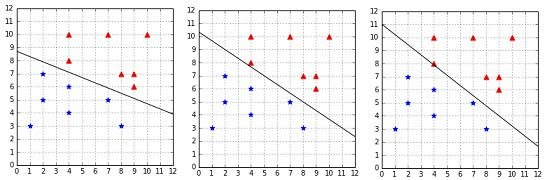
\includegraphics{figure35}
	\caption{线性可分的数据集中分别设置$C=+\infty,C=1,C=0.01$}
	\label{figure35}
\end{figure}

如果我们选择一个非常接近零的值$C$会发生什么?那么基本上就没有约束了,我们得到的超平面不能分类任何样本。

当数据是线性可分的时候,坚持用大$C$是最好的选择。但如果我们有一些嘈杂的异常值呢?在这种情况下,正如我们在图\ref{figure36}中所看到的,使用$C=+\infty$得到了一个非常窄的间隔。然而,当我们使用$C=1$时,我们得到的超平面与没有异常值下的硬间隔超平面非常接近。只有异常值违反了约束。设置$C=0.01$时则有一个非异常值违反了约束。这个$C$的值似乎给了我们的软间隔分类器太多的自由。

\begin{figure}[ht]
	\centering
	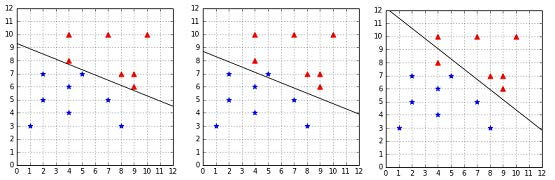
\includegraphics{figure36}
	\caption{线性可分的数据集中添加一个异常值后,分别设置$C=+\infty,C=1,C=0.01$}
	\label{figure36}
\end{figure}

最终,在异常值使数据线性不可分的情况下,我们不能使用$C=+\infty$,因为没有满足所有硬边距约束的解。相反,我们测试了$C$的几个值,并看到使用$C=3$得到了最好的超平面。事实上,我们在$C \geq 3$时得到的超平面都是一样的。这是因为无论我们如何惩罚它,都必须违反异常值的约束才能分离数据。和前面一样,当我们使用小$C$时,会违反更多的约束。

\begin{figure}[ht]
	\centering
	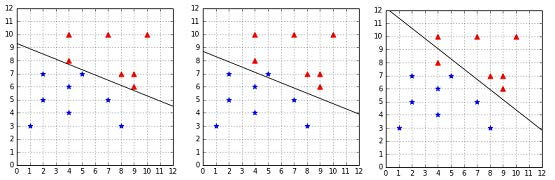
\includegraphics{figure36}
	\caption{线性不可分的数据集中,分别设置$C=3,C=1,C=0.01$}
	\label{figure36}
\end{figure}

经验法则:

* 较小的$C$会带来更大的间隔,但会存在一些错误的分类。
* 较大的$C$更接近硬间隔分类器,在这种情况下基本不能违反约束条件
* 找到噪声数据不会对解产生太大影响的$C$很关键。



\section{怎么找到最好的参数$C$}

没有任何$C$可以解决所有的问题。推荐的选择方法是使用\href{http://scikit-learn.org/stable/modules/cross_validation.html}{交叉验证}的\href{http://scikit-learn.org/stable/modules/grid_search.html}{网格搜索}(Hsu, Chang, \& Lin, A Practical Guide to Support Vector Classification)来选择$C$。要明白$C$的值非常特定于您正在使用的数据,所以如果有一天你发现$C = 0.001$不适合你的数据集,你仍然应该尝试将这个值用在另一个数据集中,因为相同的$C$在不同的数据集中完全不同。

\section{其他软间隔公式}

\subsection{2-范式软间隔(2-Norm soft margin)}

这个问题还有另一种形式,叫做2-范式(或L2正则化)软间隔,它最小化的是$\frac{1}{2} \|w\|^2 + C \sum\limits_{i=1}^m \zeta_i^2$。这个公式引出了一个没有框约束的对偶问题。关于2-范式软间隔的更多信息,请参阅(Cristianini \& shaw - taylor, 2000)。

\subsection{nu-SVM}

由于$C$的大小受特征空间的影响,所以提出了$\nu SVM$。其思想是使用一个值在0到1之间变化的参数$\nu$,而不是参数$C$。

> Note: “$\nu$为问题提供了一个更透明的参数化,它不依赖于特征空间的缩放,而只依赖于数据中的噪声水平。”(Cristianini \& Shawe-Taylor, 2000)

其所要解决的优化问题为:
\begin{gather*}
\begin{align*}
\underset{\alpha}{\text{maximize}} \quad &  - \frac{1}{2}\sum_{i=1}^m\sum_{j=1}^m \alpha_i \alpha_j y_i y_j \mathbf{x}_i \cdot \mathbf{x}_j  \\
subject\ to \quad & 0 \leq \alpha_i \leq \frac{1}{m},\text{for any }i=1,\dots,m \\
& \sum_{i=1}^m \alpha_i y_i = 0 \\
& \sum_{i=1}^m \alpha_i \geq \nu,i=1,\dots,m
\end{align*}
\end{gather*}
\section{总结}

相对于硬间隔分类器,软间隔支持向量机是一个很好的改进。即使有噪声数据打破线性可分性,它依然允许我们正确地分类数据。然而,这种增加的灵活性的代价是我们现在有了一个超参数$C$,我们需要为它找到一个值。我们看到改变$C$的值是如何影响间隔的,并允许分类器为了获得更大的间隔而做一些错位分类。这再次提醒我们,我们的目标是找到一种可以很好地处理新数据的假设函数。在训练数据上出现一些错误并不是一件坏事。